%%Metodología mecatrónica

\section{Marco Procedimental}

\subsection{Metodología VDI-2206}
Debido a la naturaleza de este proyecto, es necesario poder trabajarlo con una metodología que permita la integración de las diferentes disciplinas que intervienen entre sí. Es por esta razón que se ha seleccionado la metodología VDI-2206 (Figura \ref{fg}); dicha metodología posibilita afrontar el problema desde un punto de visto de diseño de ingeniería concurrente, ya que admite un desarrollo simultáneo de todos los módulos que van a comprender el sistema. Además de que es posible realizar una retroalimentación entre cada fase del proyecto. Esta metodología de modelo “V” consta de 5 pasos.(Figura \ref{fg:metodologia}).

\begin{figure}[h]
            \centering
            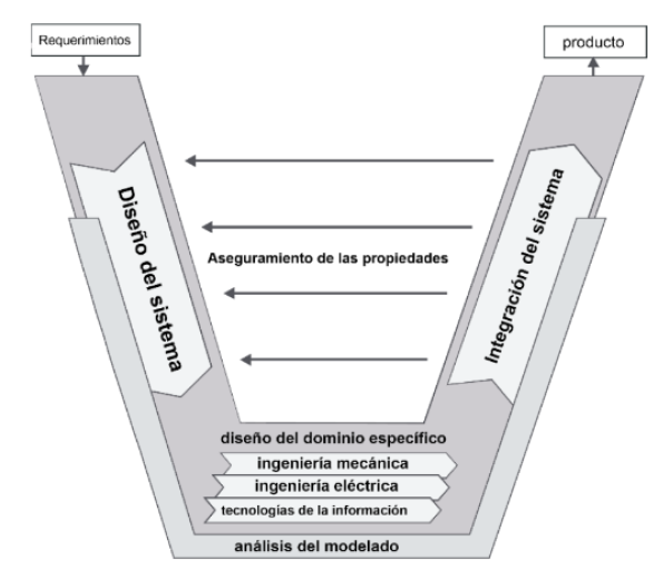
\includegraphics[scale=0.3]{images/Capitulo 1/2.2.2 Marco procedimental/VDI.png}
            \caption{Diagrama del modelo V de la metodología VDI-2206 \cite{IRI2017} }
            \label{fg:VDI}
\end{figure}



\begin{figure}[h]
            \centering
            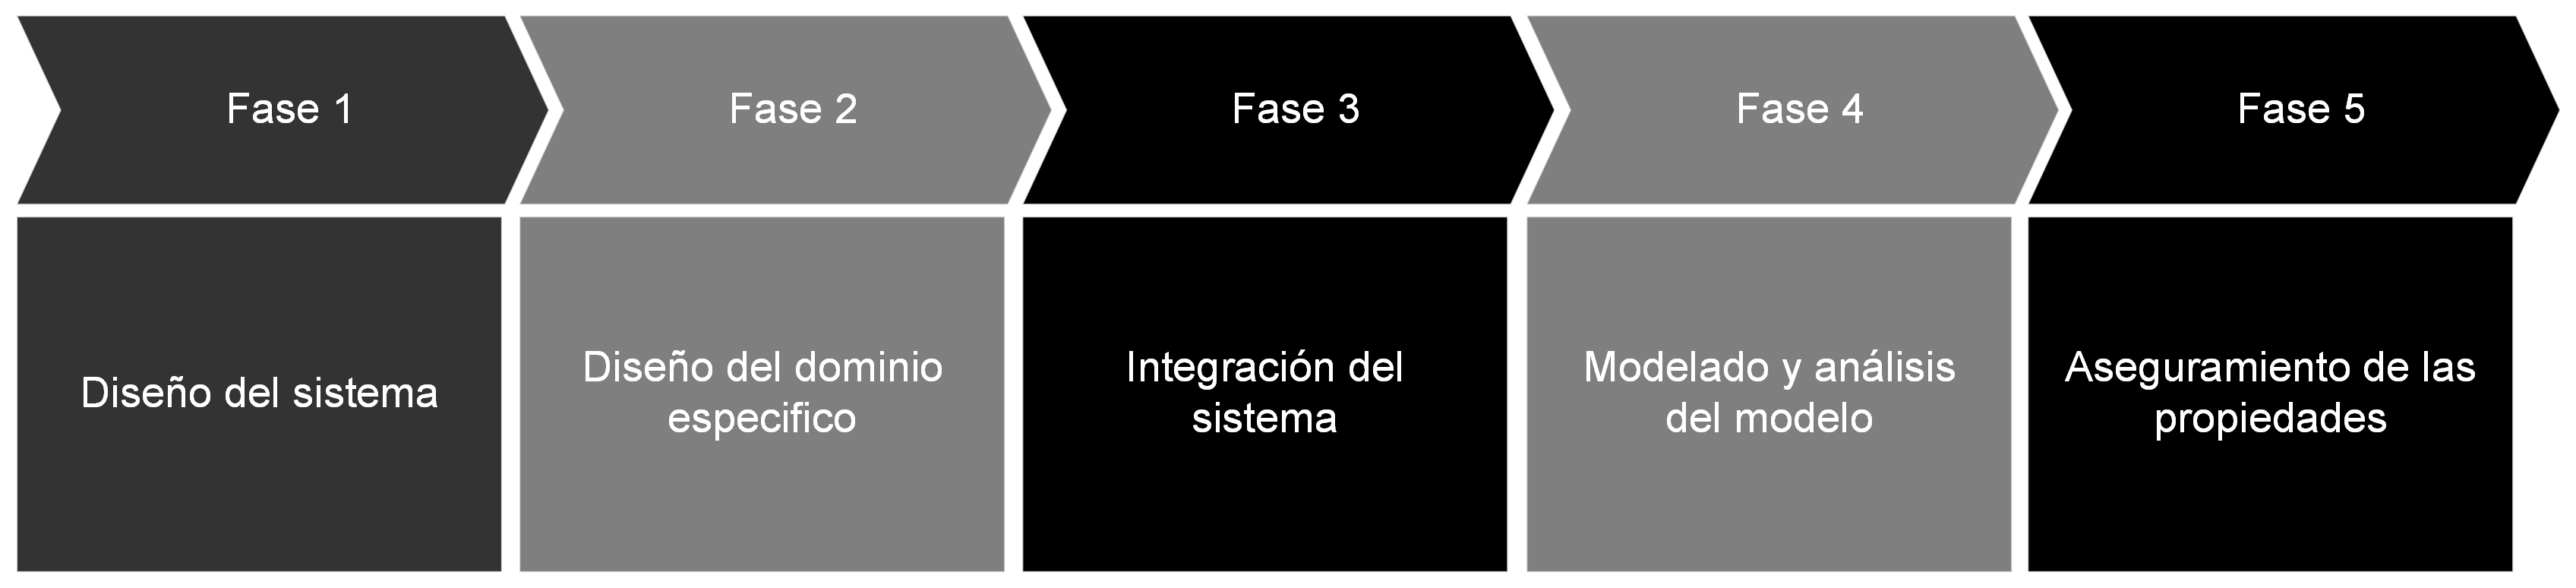
\includegraphics[scale=0.2]{images/Capitulo 1/2.2.2 Marco procedimental/Metodologia.png}
            \caption{Etapas de la metodología VDI-2206 \cite{IRI2017} }
            \label{fg:metodologia}
\end{figure}

En la primera fase, se realiza un diseño conceptual del sistema, ya que, a partir de un análisis de necesidades, se van a ir determinando los requerimientos, las funciones y la arquitectura física del sistema mecatrónico (SM). Esta etapa se ejecutará a lo largo del desarrollo de este protocolo de investigación, con el cual se sentarán las bases del proyecto. 

Es por esta razón que en esta parte del proyecto se realizarán diversos esquemas, como la Descomposición de la Estructura Funcional (FBS, por sus siglas en inglés), también el IDEF-0 para mostrar la interacción entre los módulos, que ayuden a comprender el funcionamiento general del sistema a desarrollar, en este caso, el sistema de generación de compost.
